
\section{Modelo de información del Seguimiento}

\subsection{Descripción general}
 En la figura~\ref{fig:seguimiento} se muestra la estructura de información que manejará el sistema para registrar la información del seguimiento del plan de acción.
 
\begin{figure}[htbp!]
	\begin{center}
		\fbox{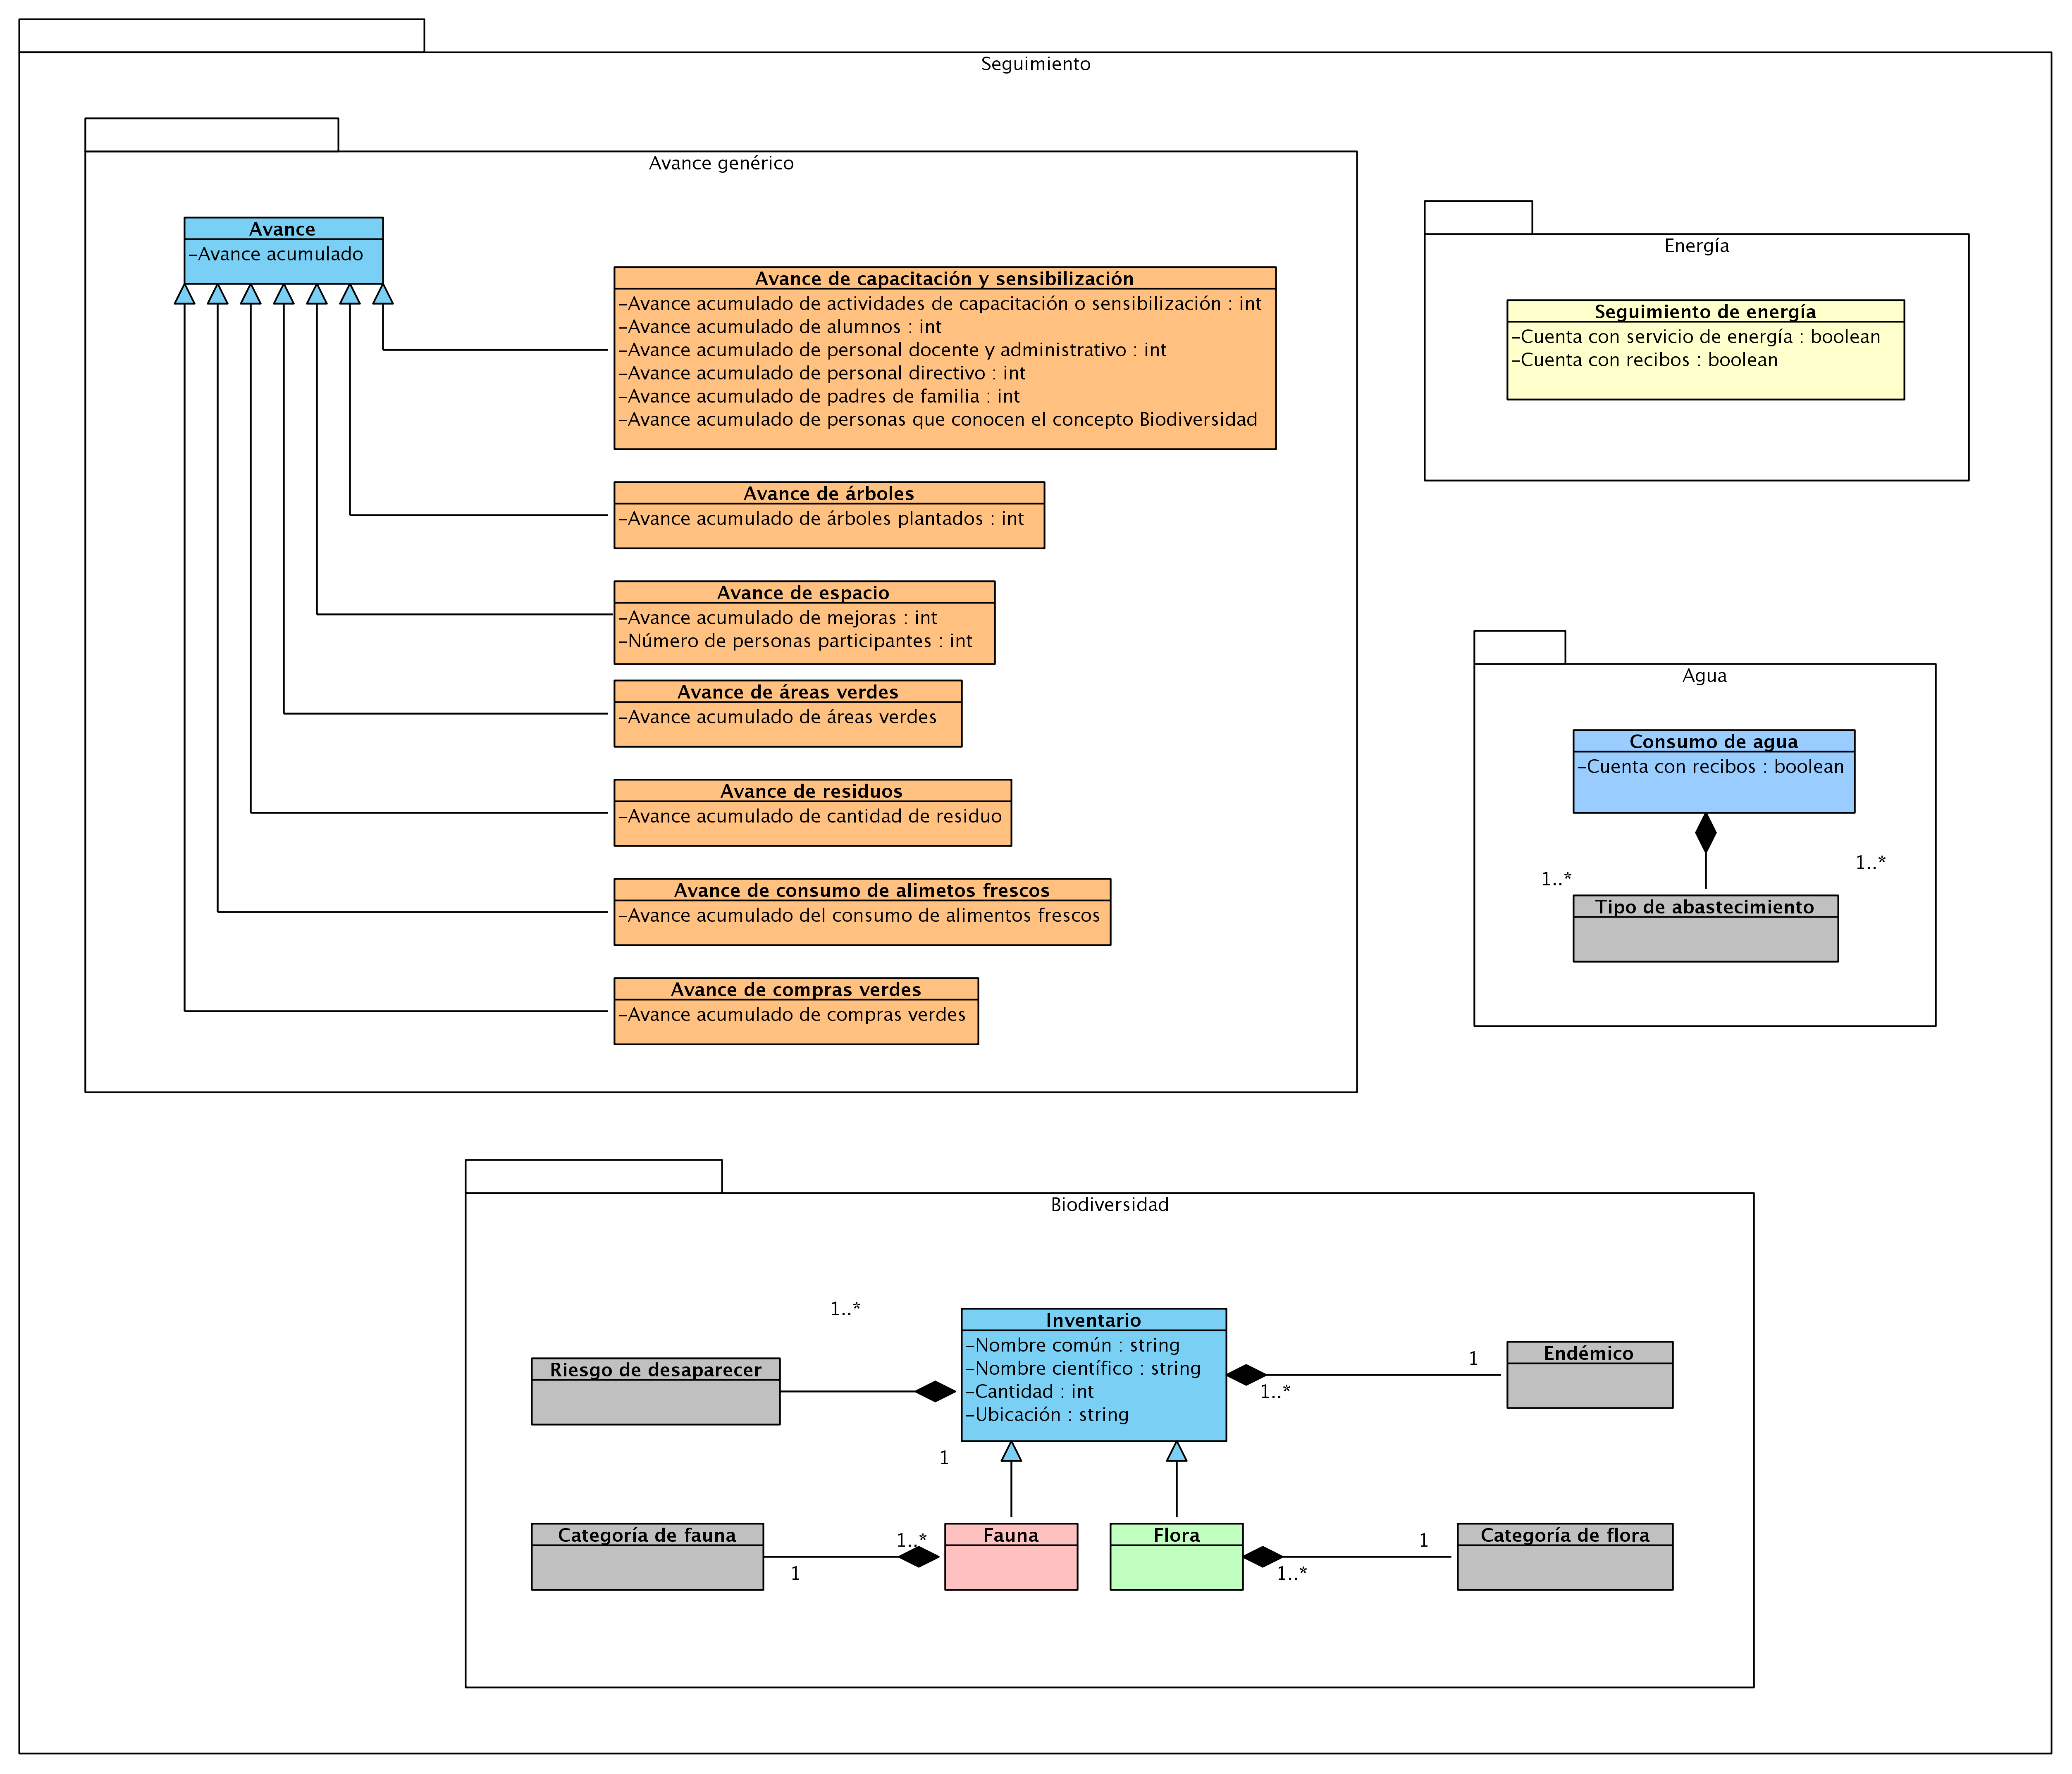
\includegraphics[width=1\textwidth]{images/clases/seguimiento}}
		\caption{Modelo de información del registro del seguimiento del plan de acción.}
		\label{fig:seguimiento}
	\end{center}
\end{figure}

%---------------------------------------
\begin{BusinessEntity}{avanceCapacitacion}{Avance de capacitación y sensibilización}
      \Battr{avanceActividades}{Avance acumulado de actividades}{\tdNumerico{entero}}{Valor acumulado resultado de la suma de los avances reportados por actividades}{\requerido}
      \Battr{avanceAlumnos}{Avance acumulado de alumnos}{\tdNumerico{entero}}{Cantidad de alumnos acumulada resultado de la suma de los avances reportados}{\requerido}
      \Battr{avanceDocenteAdministrativo}{Avance acumulado de personal docente y administrativo}{\tdNumerico{entero}}{Cantidad de personal docente y administrativo acumulada resultado de la suma de los avances reportados}{\requerido}
      \Battr{avanceDirectivos}{Avance acumulado de personal directivo}{\tdNumerico{entero}}{Cantidad de personal directivo acumulada resultado de la suma de los avances reportados}{\requerido}
      \Battr{avancePadres}{Avance acumulado de padres de familia}{\tdNumerico{entero}}{Cantidad de padres de familia acumulada resultado de la suma de los avances reportados}{\requerido}
\end{BusinessEntity}

%----------------------------------------------------------
\begin{BusinessEntity}{avanceAgua}{Avance de agua}
      \Battr{avance}{Avance acumulado de consumo de agua}{\tdNumerico{entero}}{Número de consumo de agua resultado de la suma de todos los avances reportados anteriormente}{\requerido}
\end{BusinessEntity}
%----------------------------------------------------------
\begin{BusinessEntity}{avanceArboles}{Avance de árboles}
      \Battr{avanceArboles}{Avance acumulado de árboles plantados}{\tdNumerico{entero}}{Número de árboles plantados resultado de la suma de todos los avances reportados anteriormente}{\requerido}
\end{BusinessEntity}

%----------------------------------------------------------
\begin{BusinessEntity}{avanceEspacio}{Avance de espacio}
      \Battr{avance}{Avance acumulado de mejoras}{\tdNumerico{entero}}{Cantidad de mejoras acumuladas resultado de la suma de los avances anteriores a este}{\requerido}
      \Battr{personas}{Número de personas participantes}{\tdNumerico{entero}}{Cantidad de personas que participaron en la realización de la mejora}{\requerido}
\end{BusinessEntity}

%----------------------------------------------------------
\begin{BusinessEntity}{avanceAreasVerdes}{Avance de áreas verdes}
      \Battr{avance}{Avance acumulado de áreas verdes}{\tdNumerico{entero}}{Cantidad de áreas verdes mejoradas resultado de la suma de las mejoras anteriores a esta}{\requerido}
\end{BusinessEntity}
%----------------------------------------------------------
\begin{BusinessEntity}{avanceResiduos}{Avance de residuos}
      \Battr{avance}{Avance acumulado de cantidad de residuo}{\tdNumerico{entero}}{Cantidad de residuos reciclados o reducidos, resultado de la suma de los avances reportados anteriormente}{\requerido}
\end{BusinessEntity}

%----------------------------------------------------------
\begin{BusinessEntity}{avanceAlimentos}{Avance de consumo de alimentos frescos}
      \Battr{avance}{Avance acumulado del consumo de alimentos frescos}{\tdNumerico{entero}}{Cantidad de personas que han cambiado sus hábitos alimenticios para consumir alimentos frescos}{\requerido}
\end{BusinessEntity}

%----------------------------------------------------------
\begin{BusinessEntity}{avanceComprasVerdes}{Avance de compras verdes}
      \Battr{avance}{Avance acumulado de compras verdes}{\tdNumerico{entero}}{Cantidad acumulada de compras de productos que no dañan el ambiente}{\requerido}
\end{BusinessEntity}

\subsubsection{Modelo de información posterior al plan de acción}
Las entidades que se describen a continuación forman parte de la información de las diferentes líneas de acción posterior a la aplicación del Plan de acción. Estos datos corresponden los resultados que serán utilizados por los indicadores para medir el avance final de la escuela.

%----------------------------------------------------------
\begin{BusinessEntity}{energiaSeguimiento}{Seguimiento de energía}
      \Battr{cuentaConServicio}{Cuenta con servicio de energía}{\tdBooleano}{Indica si la escuela cuenta con servicio de energía después de haber aplicado el plan de acción}{\requerido}
      \Battr{cuentaConRecibos}{Cuenta con recibos}{\tdBooleano}{Indica si la escuela cuenta con recibos del consumo de energía del periodo en el que duró el plan de acción}{\requerido}
\end{BusinessEntity}

%----------------------------------------------------------
\begin{BusinessEntity}{consumo-aguaSeguimiento}{Consumo de agua}
      \Battr{recibos}{Cuenta con recibos}{\tdBooleano}{Indica si la escuela cuenta con recibos del consumo de agua después de haber aplicado el plan de acción}{\requerido}
      %\Battr{consumoAnual}{Consumo anual promedio}{\tdNumerico{decimal}}{Cantidad promedio de agua consumida anualmente expresada en metros cúbicos}{\requerido}
      %\Battr{importeAnual}{Importe anual promedio}{\tdNumerico{decimal}}{Valor anual en pesos mexicanos del consumo anual de agua}{\requerido}
      \Battr{tipoAbastecimiento}{Tipo de abastecimiento}{\tdCatalogo}{Método empleado para transportar y suministrar el agua a la escuela, definido por el catálogo \cdtRef{gls:tipoAbastecimiento}{Tipo de abastecimiento}}{\requerido}
\end{BusinessEntity}

%----------------------------------------------------------
\begin{BusinessEntity}{inventarioSeguimiento}{Inventario}
      \Battr{nombreComun}{Nombre común}{\tdFrase}{El que se aplica a flora o fauna que pertenece a una misma clase, especie o familia, y con el que se conoce de forma popular}{\requerido}
      \Battr{nombreCientifico}{Nombre científico}{\tdFrase}{Nombre que dentro de la comunidad científica se da a las diferentes especies de plantas o animales}{\requerido}
      \Battr{cantidad}{Cantidad}{\tdNumerico{entero}}{Número de estas especies de flora o fauna con las que cuenta la escuela}{\requerido}
      \Battr{ubicacion}{Ubicación}{\tdParrafo}{Descripción del lugar en donde se encuentra la especie de flora o fauna}{\requerido}
      \Battr{riesgo}{Riesgo de desaparecer}{\tdCatalogo}{Indica si la especie de flora o fauna está en riesgo de desaparecer de la región, definido por el catálogo \cdtRef{gls:riesgo}{Riesgo de desaparecer}}{\requerido}
      \Battr{endemico}{Endémico}{\tdCatalogo}{Indica si la especie de flora o fauna es endémica, definido por el catálogo \cdtRef{gls:endemico}{Endémico}}{\requerido}
\end{BusinessEntity}

\subsubsection{Relaciones}

\begin{BusinessFact}{inventario:fauna}{Fauna}
	\BRitem{Descripción}{Fauna es un tipo de \cdtRef{inventario}{Inventario}}
	\BRitem{Tipo}{\relHerencia}
\end{BusinessFact}

\begin{BusinessFact}{inventario:flora}{Flora}
	\BRitem{Descripción}{Flora es un tipo de \cdtRef{inventario}{Inventario}}
	\BRitem{Tipo}{\relHerencia}
\end{BusinessFact}

\begin{BusinessEntity}{fauna}{Fauna}
      \Battr{categoriaFauna}{Categoría de fauna}{\tdCatalogo}{Clase a la que pertenece la especie animal, definido por el catálogo \cdtRef{gls:categoriaFauna}{Categoría de fauna}}{\requerido}
\end{BusinessEntity}

\begin{BusinessEntity}{flora}{Flora}
      \Battr{categoriaFlora}{Categoría de flora}{\tdCatalogo}{Clase a la que pertenece la especie de planta, definido por el catálogo \cdtRef{gls:categoriaFlora}{Categoría de flora}}{\requerido}
\end{BusinessEntity}